\begin{opgavetekst}{Problem 1}
\end{opgavetekst}
\begin{delopgave}{1}
	Solve for $x$ in $x^2 + y^2 = z^2$
\end{delopgave}
\begin{delopgave}{2}
	Solve for $q$ in $\sqrt{qb}=s$
\end{delopgave}
\begin{delopgave}{3}
	Solve for $m$ in $\frac{m+s}{a+r}=v$
\end{delopgave}
%
%
%
%
%
%
\begin{opgavetekst}{Problem 2}
	A line $l$ passes through the points $(2,5)$ and $(6,-11)$. 
\end{opgavetekst}
\begin{delopgave}{1}
	Determine the equation for $l$ on slope-intercept form ($y = mx + b$).
\end{delopgave}
\begin{delopgave}{2}
	Determine the equation for the line $m$ which is perpendicular to $l$ and has $x$-intercept when $x = 3$
\end{delopgave}
%
%
%
%
%
\begin{opgavetekst}{Problem 3}
\end{opgavetekst}
\begin{delopgave}{1}
	Determine the largest possible domain of each of the following functions.
	\begin{align*}
		&1) \ f(x) = \frac{1}{4x - 12} &    &2) \ g(x) = \sqrt{x - 4} \\
		&3) \ h(x) = \sqrt{x^2 - 16} &    &4) \ \varphi(x) = \ln(x^4)	
	\end{align*}	 
\end{delopgave}
%
%
%
%
%
\begin{opgavetekst}{Problem 4}
	The functions $f$ and $g$ are given as
	\begin{align*}
		f(x) = x^2-4x+2
	\end{align*}
	and
	\begin{align*}
		g(x) = 5x-3.
	\end{align*}
\end{opgavetekst}
\begin{delopgave}{1}
	Determine the following:
		\begin{align*}
		&1) \ f \circ g(1) \ &  &2) g \circ f(4) \\
		&3) \ f \circ f(1) \ &   &4) g \circ g (-4)
	\end{align*}
\end{delopgave}
%
%
%
%
%
\begin{opgavetekst}{Problem 5}
	The functions $p$ and $q$ are given as
	\begin{align*}
		p(x) = \sqrt{x - 1}
	\end{align*}
	and 
	\begin{align*}
		q(x) = 2^x
	\end{align*}
\end{opgavetekst}
\begin{delopgave}{1}
	Determine an expression for the composite functions $f\circ g$ and $g \circ f$
\end{delopgave}
%
%
%
%
%
\begin{opgavetekst}{Problem 6}
	Check whether the following pairs of functions are mutually inverse. 
\end{opgavetekst}
\begin{delopgave}{1}
	$f(x) = 2x + 4$ and $g(x) = \frac{x-4}{2}$.
\end{delopgave}
\begin{delopgave}{2}
	$f(x) = \sqrt{x-1}$ and $g(x) = x^2 - 1$.
\end{delopgave}
\begin{delopgave}{3}
	$f(x) = 2^{3x - 10}$ and $g(x) = \log_{2}\left(\frac{x+10}{3}\right)$.
\end{delopgave}
\begin{delopgave}{4}
	$f(x) = e^{\sqrt{x}}$ and $g(x) = \ln(x)^2$.
\end{delopgave}
%
%
%
%
%
\newpage
\begin{opgavetekst}{Problem 7}
	A one-to-one function $f$ is given by
	\begin{align*}	
		f(x) = e^{\frac{x^3-9}{2}}
	\end{align*}
\end{opgavetekst}
\begin{delopgave}{1}
	Determine an expression for the inverse $f^{-1}$.
\end{delopgave}
%
%
%%%%%%%%%%%%%%%
%
%
\begin{opgavetekst}{Problem 8}
A function $f^{-1}$ is given by the following graph.\\
\begin{center}
\resizebox{0.45\textwidth}{!}{
	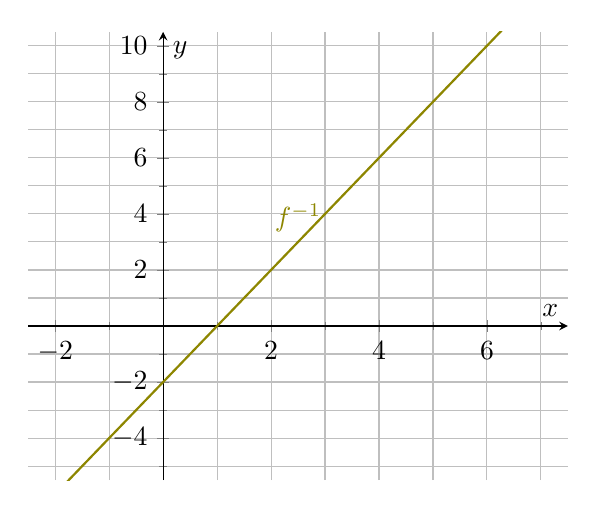
\begin{tikzpicture}
	\begin{axis}[
	axis lines = center, 
	xmin = -2.5, xmax = 7.5,
	ymin = -5.5, ymax = 10.5,
	xlabel = $x$, 
	ylabel = $y$,
	xtick = {-4,-2,...,6,8},
	ytick = {-8,-6,...,10,12},
	minor tick num = 1,
	grid = both,
	]
		\addplot[color = olive, thick, samples = 500, domain = -10:10] {2*x-2};
		\node[color = olive, anchor = south] at (axis cs: 2.5,3) {$f^{-1}$};
	\end{axis}
	\end{tikzpicture}
	}
\end{center}
\phantom{h}
\end{opgavetekst}
\begin{delopgave}{1}
	Determine $f^{-1}(1)$.
\end{delopgave}
\begin{delopgave}{2}
	Determine $f(4)$.
\end{delopgave}
\begin{delopgave}{3}
	Solve the equation $f^{-1}(x) = 8$.
\end{delopgave}
\begin{delopgave}{4}
	Solve the equation $f(x) = 4$.
\end{delopgave}
%
%
%%%%%%%%%%%%%%%
%
%
\begin{opgavetekst}{Problem 9}
	A colony of bacteria contains 1.4 billion bacteria. The number of bacteria increases $11.2\%$ per day.
\end{opgavetekst}
\begin{delopgave}{1}
	Determine an expression that yields the number of bacteria (in billions) as a function of the number of 
	days passed. 
\end{delopgave}
\begin{delopgave}{2}
	Determine the number of bacteria after 20 days. Use your GCD. 
\end{delopgave}
%
%
%%%%%%%%%%%%%%%
%
%
\newpage
\begin{opgavetekst}{Problem 10}
	You invest 75$\TS$000 in an account with a yearly interest of $4.2$ percent.  
\end{opgavetekst}
\begin{delopgave}{1}
	Determine the value of the investment after 15 years if the interest is compounded annualy
\end{delopgave}
\begin{delopgave}{2}
	Determine the value of the investment after 10 years if the interest is compounded monthly, weekly
	and daily	
\end{delopgave}
%
%
%%%%%%%%%%%%%%%
%
%
\begin{opgavetekst}{Problem 11}
	An exponential function $f$ is given as
	\begin{align*}
		f(x) = b\cdot a^x
	\end{align*}
	and passes through the points $(2,3)$ and $(4,9)$. 
\end{opgavetekst}
\begin{delopgave}{1}
	Determine the value of $a$ and $b$. (Hint: Evaluate $f$ at the points and divide the expressions for $f$. )
\end{delopgave}
%
%
%%%%%%%%%%%%%%%
%
%
\begin{opgavetekst}{Problem 12}
\end{opgavetekst}
\begin{delopgave}{1}
	Determine the value of the following logarithmic expressions
	\begin{align*}
		&1) \ \log_{5}(125)& &2) \ \log_{7}\left(\frac{1}{49}\right)\\
		&3) \ \log_{2}(1024)& &4) \ \log_{64}(16)\\
		&5) \ \log_{10}(0.00001)& &6) \ \log_{27}(3)\\
		&7) \ \ln(e^{-0.3})& &8) \ \log_{128}(8)\\
	\end{align*}
\end{delopgave}
